\begin{frame}[label=Oresme]
  \frametitle{Oresme}
    Nel 1361,il matematico Oresme rappresentò il moto con una serie
    di grafici in cui \alert{la velocità} dipendeva dal \alert{tempo}.
    \begin{center}
    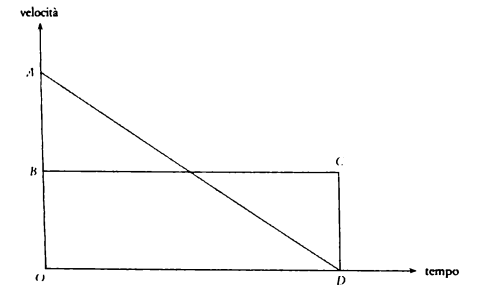
\includegraphics[scale=.4]{Oresme.png}    
    \end{center}
    \pause
    Egli dedusse che la distanza percorsa da un corpo \textit{A} che si muove con 
    accelerazione costante è pari a quella di un corpo \textit{B} che si muove con 
    velocità costante pari alla media delle velocità iniziale e finale del corpo \textit{A}.
    \pause
    \begin{block}{TFC secondo Oresme}
      Oresme assume che la distanza percorsa da un corpo qualsiasi è pari
      all' \alert{area} sottesa dal grafico velocità-tempo.
    \end{block}  
  
  \end{frame}